\newpage
\section{Anhang}




\subsection{Tabellen}

\subsubsection{Messdaten Drehschieberpumpe}

\begin{table}[H]
\tiny
\centering
\begin{tabular}{S [table-format=3.0] S [table-format=2.3] S [table-format=2.3] S [table-format=2.3] c c }
    \toprule
    \multicolumn{1}{p{3.2cm}}{\centering$\text{t} $\\$ \text{in } \si{\second} $ } &
    \multicolumn{1}{p{3.2cm}}{\centering$\text{Druck Messreihe 1 } $\\$ \text{in }\si{\milli\bar}$} &
    \multicolumn{1}{p{3.2cm}}{\centering$\text{Druck Messreihe 2 } $\\$ \text{in }\si{\milli\bar}$} &
    \multicolumn{1}{p{3.2cm}}{\centering$\text{Druck Messreihe 3 } $\\$ \text{in }\si{\milli\bar}$} &
    \multicolumn{1}{p{3.2cm}}{\centering$\text{Druck gemittelt } $\\$ \text{in }\si{\milli\bar}$} &
    \multicolumn{1}{p{3.2cm}}{\centering$ \ln{\frac{p(t) - p_{end}}{p_0 - p_{end}}}$}\\
    \midrule
    0  &  995.1  & 995.4  & 989.7  & 993.4  \pm 1.5      &     0.0 \pm 0                                    \\
    10  & 644    & 640    & 640    & 641.3  \pm 1.1      & -0.4376 \pm 0.0022                           \\
    20  & 479    & 439    & 477    & 465    \pm 11       & -0.7592 \pm 0.0028                             \\
    30  & 358    & 327    & 357    & 347    \pm 8        &  -1.051 \pm 0.004                               \\
    40  & 265    & 236    & 266    & 256    \pm 8        &  -1.357 \pm 0.005                               \\
    50  & 201    & 177    & 196    & 191    \pm 6        &  -1.647 \pm 0.006                               \\
    60  & 147    & 131    & 144    & 141    \pm 4        &  -1.955 \pm 0.009                               \\
    70  & 103    &  95    & 108    & 102.0  \pm 3.1      &  -2.277 \pm 0.012                             \\
    80  &  75    &  69.8  &  76.9  & 73.9   \pm 1.7      &  -2.599 \pm 0.016                              \\
    90  &  55    &  51    &  56.2  & 54.1   \pm 1.3      &  -2.912 \pm 0.022                              \\
    100  & 40.2  &  36.7  &  41.1  & 39.3   \pm 1.1      &  -3.230 \pm 0.031                              \\
    110  & 29.9  &  26.4  &  30.3  & 28.9   \pm 1.0      &  -3.54  \pm 0.04                                \\
    120  & 21.5  &  19.1  &  21.4  & 20.7   \pm 0.6      &  -3.87  \pm 0.06                                \\
    130  & 15.1  &  14    &  15.5  & 14.9   \pm 0.4      &  -4.21  \pm 0.08                                \\
    140  & 10.8  &  10    &  11.3  & 10.70  \pm 0.31     &  -4.54  \pm 0.11                               \\
    150  &  7.9  &   7.3  &   8.5  & 7.90   \pm 0.28     &  -4.841 \pm 0.034                              \\
    160  &  5.9  &   5.5  &   6.1  & 5.83   \pm 0.14     &  -5.146 \pm 0.034                              \\
    170  &  4.5  &   4.2  &   4.6  & 4.43   \pm 0.10     &  -5.423 \pm 0.034                              \\
    180  &  3.5  &   3.2  &   3.6  & 3.43   \pm 0.10     &  -5.682 \pm 0.034                              \\
    190  &  2.8  &   2.6  &   2.9  & 2.77   \pm 0.07     &  -5.902 \pm 0.034                              \\
    200  &  2.2  &   2.1  &   2.3  & 2.20   \pm 0.05     &  -6.136 \pm 0.034                              \\
    210  &  1.9  &   1.6  &   1.9  & 1.80   \pm 0.08     &  -6.341 \pm 0.034                              \\
    220  &  1.6  &   1.5  &   1.6  & 1.567  \pm 0.027    &  -6.485 \pm 0.034                             \\
    230  &  1.4  &   1.3  &   1.4  & 1.367  \pm 0.027    &  -6.626 \pm 0.035                             \\
    240  &  1.2  &   1.2  &   1.2  & 1.2    \pm 0        &  -6.761 \pm 0.035                               \\
    250  &  1    &   0.99 &   1.1  & 1.030  \pm 0.029    &  -6.921 \pm 0.035                             \\
    260  &  0.93 &   0.91 &   0.94 & 0.927  \pm 0.007    &  -7.033 \pm 0.035                             \\
    270  &  0.83 &   0.82 &   0.86 & 0.837  \pm 0.010    &  -7.14  \pm 0.04                               \\
    280  &  0.76 &   0.74 &   0.77 & 0.757  \pm 0.007    &  -7.25  \pm 0.04                               \\
    290  &  0.68 &   0.67 &   0.7  & 0.683  \pm 0.007    &  -7.36  \pm 0.04                               \\
    300  &  0.63 &   0.62 &   0.64 & 0.630  \pm 0.005    &  -7.45  \pm 0.04                               \\
    310  &  0.59 &   0.57 &   0.6  & 0.587  \pm 0.007    &  -7.52  \pm 0.04                               \\
    320  &  0.54 &   0.53 &   0.55 & 0.540  \pm 0.005    &  -7.61  \pm 0.04                               \\
    330  &  0.5  &   0.5  &   0.51 & 0.503  \pm 0.0027   &  -7.69  \pm 0.04                              \\
    340  &  0.47 &   0.46 &   0.47 & 0.4667 \pm 0.0027   &  -7.78  \pm 0.04                              \\
    350  &  0.44 &   0.43 &   0.44 & 0.4367 \pm 0.0027   &  -7.85  \pm 0.04                              \\
    360  &  0.41 &   0.41 &   0.42 & 0.4133 \pm 0.0027   &  -7.91  \pm 0.04                              \\
    370  &  0.39 &   0.39 &   0.4  & 0.3933 \pm 0.0027   &  -7.97  \pm 0.04                              \\
    380  &  0.37 &   0.36 &   0.38 & 0.370  \pm 0.005    &  -8.04  \pm 0.04                               \\
    390  &  0.35 &   0.35 &   0.35 & 0.350  \pm 0         &  -8.11 \pm 0.04                               \\
    400  &  0.33 &   0.33 &   0.33 & 0.33   \pm 0        &  -8.17  \pm 0.04                                \\
    410  &  0.31 &   0.31 &   0.32 & 0.3133 \pm 0.0027   &  -8.24  \pm 0.04                              \\
    420  &  0.3  &   0.3  &   0.3  & 0.3    \pm 0        &  -8.29  \pm 0.04                                 \\
    430  &  0.28 &   0.28 &   0.29 & 0.2833 \pm 0.0027   &  -8.36  \pm 0.04                              \\
    440  &  0.27 &   0.27 &   0.28 & 0.2733 \pm 0.0027   &  -8.40  \pm 0.04                              \\
    450  &  0.26 &   0.26 &   0.27 & 0.2633 \pm 0.0027   &  -8.45  \pm 0.04                              \\
    460  &  0.25 &   0.25 &   0.25 & 0.25   \pm 0        &  -8.51  \pm 0.04                                \\
    470  &  0.24 &   0.24 &   0.24 & 0.24   \pm 0        &  -8.56  \pm 0.04                                \\
    480  &  0.23 &   0.23 &   0.23 & 0.23   \pm 0        &  -8.62  \pm 0.04                                \\
    490  &  0.21 &   0.22 &   0.23 & 0.220  \pm 0.005    &  -8.67  \pm 0.04                               \\
    500  &  0.21 &   0.21 &   0.21 & 0.21   \pm 0        &  -8.73  \pm 0.04                                \\
    510  &  0.2  &   0.2  &   0.21 & 0.2033 \pm 0.0027   &  -8.78  \pm 0.05                              \\
    520  &  0.19 &   0.2  &   0.2  & 0.1967 \pm 0.0027   &  -8.82  \pm 0.05                              \\
    530  &  0.18 &   0.19 &   0.19 & 0.1867 \pm 0.0027   &  -8.89  \pm 0.05                              \\
    540  &  0.17 &   0.18 &   0.18 & 0.1767 \pm 0.0027   &  -8.97  \pm 0.05                              \\
    550  &  0.17 &   0.18 &   0.18 & 0.1767 \pm 0.0027   &  -8.97  \pm 0.05                              \\
    560  &  0.16 &   0.17 &   0.17 & 0.1667 \pm 0.0027   &  -9.05  \pm 0.05                              \\
    570  &  0.16 &   0.16 &   0.16 & 0.16   \pm 0        &  -9.11  \pm 0.05                                \\
    580  &  0.15 &   0.16 &   0.16 & 0.1567 \pm 0.0027   &  -9.14  \pm 0.05                              \\
    590  &  0.15 &   0.15 &   0.15 & 0.15   \pm 0        &  -9.20  \pm 0.05                                \\
    600  &  0.14 &   0.15 &   0.15 & 0.1467 \pm 0.0027   &  -9.24  \pm 0.05                              \\
         & 0.05 &   0.05 &   0.05 & 0.05   \pm  0       &                                   \\
    \bottomrule 
    \end{tabular}
    \caption{Messwerte der Drehschieberpumpenmessreihen für die Druckkurve.}
    \label{tab:dreh_p}
\end{table}



    \begin{table}[H]
        \centering
        \begin{tabular}{S [table-format=3.0] S [table-format=2.3] S [table-format=2.3] S [table-format=2.3] c }
            \toprule
            \multicolumn{1}{p{3.2cm}}{\centering$\text{t} $\\$ \text{in } \si{\second} $ } &
            \multicolumn{1}{p{3.2cm}}{\centering$\text{Druck Messreihe 1 } $\\$ \text{in }\si{\milli\bar}$} &
            \multicolumn{1}{p{3.2cm}}{\centering$\text{Druck Messreihe 2 } $\\$ \text{in }\si{\milli\bar}$} &
            \multicolumn{1}{p{3.2cm}}{\centering$\text{Druck Messreihe 3 } $\\$ \text{in }\si{\milli\bar}$} &
            \multicolumn{1}{p{3.2cm}}{\centering$\text{Druck gemittelt } $\\$ \text{in }\si{\milli\bar}$} \\
            \midrule
            0  &   0.39 & 0.39 & 0.39 & 0.39  \pm 0 \\
            10  &  1.3  & 1.4  & 1.3  & 1.333 \pm 0.027                               \\
            20  &  1.4  & 1.5  & 1.4  & 1.433 \pm 0.027                               \\
            30  &  1.5  & 1.5  & 1.5  & 1.5   \pm 0                                     \\
            40  &  1.6  & 1.6  & 1.6  & 1.6   \pm 0  \\
            50  &  1.6  & 1.6  & 1.6  & 1.6   \pm 0  \\
            60  &  1.7  & 1.7  & 1.7  & 1.7   \pm 0                                     \\
            70  &  1.8  & 1.8  & 1.8  & 1.8   \pm 0                                     \\
            80  &  1.9  & 1.9  & 1.9  & 1.9   \pm 0  \\
            90  &  1.9  & 1.9  & 1.9  & 1.9   \pm 0   \\
            100  & 2    & 2    & 2    & 2.0   \pm 0                                     \\
            110  & 2.1  & 2.1  & 2.1  & 2.1   \pm 0                                     \\
            120  & 2.1  & 2.2  & 2.1  & 2.133 \pm 0.027                               \\
            130  & 2.2  & 2.2  & 2.2  & 2.2   \pm 0                                     \\
            140  & 2.3  & 2.3  & 2.2  & 2.267 \pm 0.027                               \\
            150  & 2.3  & 2.4  & 2.3  & 2.333 \pm 0.027                               \\
            160  & 2.4  & 2.5  & 2.4  & 2.433 \pm 0.027                               \\
            170  & 2.5  & 2.5  & 2.5  & 2.5   \pm 0                                     \\
            180  & 2.6  & 2.6  & 2.6  & 2.6   \pm 0                                     \\
            190  & 2.7  & 2.7  & 2.6  & 2.667 \pm 0.027                               \\
            200  & 2.7  & 2.8  & 2.7  & 2.733 \pm 0.027                               \\
            \bottomrule 
            \end{tabular}
            \caption{Messwerte der Leckratenmessung für den Gleichgewichtsdruck $\SI{0.4}{\milli\bar}$ mit der Drehschieberpumpe.}
            \label{tab:dreh_leck_1}
    \end{table}

    \begin{table}[H]
        \centering
        \begin{tabular}{S [table-format=3.0] S [table-format=2.3] S [table-format=2.3] S [table-format=2.3] c }
            \toprule
            \multicolumn{1}{p{3.2cm}}{\centering$\text{t} $\\$ \text{in } \si{\second} $ } &
            \multicolumn{1}{p{3.2cm}}{\centering$\text{Druck Messreihe 1 } $\\$ \text{in }\si{\milli\bar}$} &
            \multicolumn{1}{p{3.2cm}}{\centering$\text{Druck Messreihe 2 } $\\$ \text{in }\si{\milli\bar}$} &
            \multicolumn{1}{p{3.2cm}}{\centering$\text{Druck Messreihe 3 } $\\$ \text{in }\si{\milli\bar}$} &
            \multicolumn{1}{p{3.2cm}}{\centering$\text{Druck gemittelt } $\\$ \text{in }\si{\milli\bar}$} \\
            \midrule
            0  &   10   & 10   & 10   & 10.0   \pm 0       \\
            10  &  19.3 & 19.3 & 19.2 & 19.267 \pm 0.027 \\
            20  &  23.1 & 23.1 & 22.9 & 23.03  \pm 0.05   \\
            30  &  26.8 & 26.8 & 26.8 & 26.8   \pm 0       \\
            40  &  30.3 & 30.3 & 30.4 & 30.333 \pm 0.027 \\
            50  &  34.2 & 34.2 & 34.1 & 34.167 \pm 0.027 \\
            60  &  38   & 38   & 37.8 & 37.93  \pm 0.05   \\
            70  &  41.5 & 41.5 & 41.6 & 41.533 \pm 0.027 \\
            80  &  45.5 & 45.5 & 45.3 & 45.43  \pm 0.05   \\
            90  &  48.9 & 48.9 & 49.1 & 48.97  \pm 0.05   \\
            100  & 53   & 53   & 52.8 & 52.93  \pm 0.05   \\
            110  & 56   & 56   & 56.6 & 56.20  \pm 0.16   \\
            120  & 60.5 & 60.5 & 60.3 & 60.43  \pm 0.05   \\
            130  & 63.8 & 63.8 & 64   & 63.87  \pm 0.05   \\
            140  & 67.5 & 67.5 & 68.1 & 67.70  \pm 0.16   \\
            150  & 71.5 & 71.5 & 71.1 & 71.37  \pm 0.11   \\
            160  & 75   & 75   & 75.2 & 75.07  \pm 0.05   \\
            170  & 78.8 & 78.8 & 79.2 & 78.93  \pm 0.11   \\
            180  & 82.8 & 82.8 & 82.6 & 82.73  \pm 0.05   \\
            190  & 86.8 & 86.6 & 86.2 & 86.53  \pm 0.14   \\
            200  & 90.2 & 90.2 & 90.1 & 90.167 \pm 0.027 \\
            \bottomrule 
            \end{tabular}
            \caption{Messwerte der Leckratenmessung für den Gleichgewichtsdruck $\SI{10}{\milli\bar}$ mit der Drehschieberpumpe.}
            \label{tab:dreh_leck_2}
    \end{table}

    \begin{table}[H]
        \centering
        \begin{tabular}{ S [table-format=3.0] S [table-format=3.3] S [table-format=3.3] S [table-format=3.3] c }
            \toprule
            \multicolumn{1}{p{3.2cm}}{\centering$\text{t} $\\$ \text{in } \si{\second} $ } &
            \multicolumn{1}{p{3.2cm}}{\centering$\text{Druck Messreihe 1 } $\\$ \text{in }\si{\milli\bar}$} &
            \multicolumn{1}{p{3.2cm}}{\centering$\text{Druck Messreihe 2 } $\\$ \text{in }\si{\milli\bar}$} &
            \multicolumn{1}{p{3.2cm}}{\centering$\text{Druck Messreihe 3 } $\\$ \text{in }\si{\milli\bar}$} &
            \multicolumn{1}{p{3.2cm}}{\centering$\text{Druck gemittelt } $\\$ \text{in }\si{\milli\bar}$} \\
            \midrule
            0  &    40.1 &  40.2 &  40.1 & 40.133 \pm 0.027 \\
            10  &   61.7 &  61.4 &  61.4 & 61.50  \pm 0.08   \\
            20  &   75.8 &  75.5 &  75.5 & 75.60  \pm 0.08   \\
            30  &   90   &  89.5 &  89.6 & 89.70  \pm 0.12   \\
            40  &  104   & 103.7 & 103.7 & 103.80 \pm 0.08  \\
            50  &  118.2 & 117.8 & 117.8 & 117.93 \pm 0.11  \\
            60  &  133.2 & 131.9 & 131.8 & 132.3  \pm 0.4    \\
            70  &  146.4 & 145.9 & 145.9 & 146.07 \pm 0.14  \\
            80  &  160.5 & 160.1 & 159.9 & 160.17 \pm 0.14  \\
            90  &  174.5 & 174.1 & 174   & 174.20 \pm 0.12  \\
            100  & 188.7 & 188.2 & 188.1 & 188.33 \pm 0.15  \\
            110  & 202.1 & 201.5 & 201.4 & 201.67 \pm 0.18  \\
            120  & 216.1 & 215.6 & 215.5 & 215.73 \pm 0.15  \\
            130  & 230.2 & 229.8 & 229.5 & 229.83 \pm 0.17  \\
            140  & 244.3 & 245.3 & 243.7 & 244.4  \pm 0.4    \\
            150  & 258.6 & 258.2 & 257.8 & 258.20 \pm 0.19  \\
            160  & 274.1 & 272.2 & 271.9 & 272.7  \pm 0.6    \\
            170  & 286.7 & 285.3 & 285.9 & 285.97 \pm 0.33  \\
            180  & 300.8 & 303.2 & 300.1 & 301.4  \pm 0.8    \\
            190  & 315   & 314.4 & 314.2 & 314.53 \pm 0.20  \\
            200  & 329.1 & 328.5 & 328.3 & 328.63 \pm 0.20  \\
            \bottomrule 
            \end{tabular}
            \caption{Messwerte der Leckratenmessung für den Gleichgewichtsdruck $\SI{40}{\milli\bar}$ mit der Drehschieberpumpe.}
            \label{tab:dreh_leck_3}
    \end{table}

    \begin{table}[H]
        \centering
        \begin{tabular}{S [table-format=3.0] S [table-format=2.3] S [table-format=2.3] S [table-format=2.3] c }
            \toprule
            \multicolumn{1}{p{3.2cm}}{\centering$\text{t} $\\$ \text{in } \si{\second} $ } &
            \multicolumn{1}{p{3.2cm}}{\centering$\text{Druck Messreihe 1 } $\\$ \text{in }\si{\milli\bar}$} &
            \multicolumn{1}{p{3.2cm}}{\centering$\text{Druck Messreihe 2 } $\\$ \text{in }\si{\milli\bar}$} &
            \multicolumn{1}{p{3.2cm}}{\centering$\text{Druck Messreihe 3 } $\\$ \text{in }\si{\milli\bar}$} &
            \multicolumn{1}{p{3.2cm}}{\centering$\text{Druck gemittelt } $\\$ \text{in }\si{\milli\bar}$} \\
            \midrule
            0  &   80   &  80   &  80   & 80.0    \pm 0      \\
            10  &  116.9 & 116   & 115.9 & 116.27 \pm 0.26 \\
            20  &  143.9 & 143.1 & 143.1 & 143.37 \pm 0.22 \\
            30  &  171   & 170.3 & 170   & 170.43 \pm 0.24 \\
            40  &  198   & 197.3 & 196.8 & 197.37 \pm 0.28 \\
            50  &  224   & 223.4 & 225.9 & 224.4  \pm 0.6   \\
            60  &  251.1 & 252.1 & 253   & 252.1  \pm 0.4   \\
            70  &  178.2 & 280   & 280   & 246    \pm 28      \\
            80  &  305.2 & 307.1 & 307.2 & 306.5  \pm 0.5   \\
            90  &  332.3 & 334.2 & 334.2 & 333.6  \pm 0.5   \\
            100  & 359.4 & 361.3 & 361.2 & 360.6  \pm 0.5   \\
            110  & 386.2 & 388.1 & 488.1 & 421    \pm 27      \\
            120  & 413   & 415.1 & 417.1 & 415.1  \pm 1.0   \\
            130  & 439   & 441.3 & 441.7 & 440.7  \pm 0.7   \\
            140  & 466.3 & 468.3 & 468.2 & 467.6  \pm 0.5   \\
            150  & 492.8 & 494.7 & 494.2 & 493.9  \pm 0.5   \\
            160  & 518.8 & 520.7 & 520.8 & 520.1  \pm 0.5   \\
            170  & 544.8 & 546.6 & 546.7 & 546.0  \pm 0.5   \\
            180  & 570.4 & 572.3 & 572.2 & 571.6  \pm 0.5   \\
            190  & 595   & 596.4 & 597.3 & 596.2  \pm 0.5   \\
            200  & 620.8 & 620   & 622.5 & 621.1  \pm 0.6   \\
            \bottomrule 
            \end{tabular}
            \caption{Messwerte der Leckratenmessung für den Gleichgewichtsdruck $\SI{80}{\milli\bar}$ mit der Drehschieberpumpe.}
            \label{tab:dreh_leck_4}
    \end{table}



\subsubsection{Messdaten Turbomolekularpumpe}



\begin{table}[H]
    \small
    \centering
    \begin{tabular}{c c c c c c }
        \toprule
        \multicolumn{1}{p{3.2cm}}{\centering$\text{t} $\\$ \text{in } \si{\second} $ } &
        \multicolumn{1}{p{3.2cm}}{\centering$\text{Druck Messreihe 1 } $\\$ \text{in }\si{\milli\pascal}$} &
        \multicolumn{1}{p{3.2cm}}{\centering$\text{Druck Messreihe 2 } $\\$ \text{in }\si{\milli\pascal}$} &
        \multicolumn{1}{p{3.2cm}}{\centering$\text{Druck Messreihe 3 } $\\$ \text{in }\si{\milli\pascal}$} &
        \multicolumn{1}{p{3.2cm}}{\centering$\text{Druck gemittelt } $\\$ \text{in }\si{\milli\pascal}$} &
        \multicolumn{1}{p{3.2cm}}{\centering$ \ln{\frac{p(t) - p_{end}}{p_0 - p_{end}}}$}\\
        \midrule
        0  &   166    & 169    & 167    & 167.3 \pm 0.7  &   0.0 \pm 0     \\
        10  &  7.8  &   8.73 &  79.8  & 32      \pm 19   & -1.68 \pm 0.20    \\
        20  &  3.3  &   2.98 &   2.7  & 2.99    \pm 0.14 & -4.42 \pm 0.23  \\
        30  &  2.72 &   2.4  &   2.2  & 2.44    \pm 0.12 & -4.75 \pm 0.25  \\
        40  &  2.54 &   2.22 &   2.04 & 2.27    \pm 0.12 & -4.88 \pm 0.26  \\
        50  &  2.42 &   2.13 &   1.95 & 2.17    \pm 0.11 & -4.96 \pm 0.26  \\
        60  &  2.33 &   2.05 &   1.88 & 2.09    \pm 0.11 & -5.03 \pm 0.27  \\
        70  &  2.25 &   1.99 &   1.82 & 2.02    \pm 0.10 & -5.09 \pm 0.28  \\
        80  &  2.2  &   1.94 &   1.78 & 1.97    \pm 0.10 & -5.14 \pm 0.28  \\
        90  &  2.16 &   1.9  &   1.74 & 1.93    \pm 0.10 & -5.18 \pm 0.29  \\
        100  & 2.12 &   1.87 &   1.71 & 1.90    \pm 0.10 & -5.22 \pm 0.29  \\
        110  & 2.09 &   1.84 &   1.68 & 1.87    \pm 0.10 & -5.25 \pm 0.30  \\
        120  & 2.06 &   1.81 &   1.66 & 1.84    \pm 0.10 & -5.28 \pm 0.30  \\
        130  & 2.03 &   1.79 &   1.63 & 1.82    \pm 0.09 & -5.32 \pm 0.30  \\
        140  & 2.01 &   1.77 &   1.62 & 1.80    \pm 0.09 & -5.34 \pm 0.31  \\
        150  & 1.98 &   1.75 &   1.6  & 1.78    \pm 0.09 & -5.37 \pm 0.31  \\
        160  & 1.96 &   1.73 &   1.58 & 1.76    \pm 0.09 & -5.39 \pm 0.32  \\
        170  & 1.94 &   1.71 &   1.57 & 1.74    \pm 0.09 & -5.42 \pm 0.32  \\
        180  & 1.92 &   1.7  &   1.55 & 1.72    \pm 0.09 & -5.44 \pm 0.32  \\
        190  & 1.91 &   1.68 &   1.54 & 1.71    \pm 0.09 & -5.46 \pm 0.33  \\
        200  & 1.9  &   1.67 &   1.53 & 1.70    \pm 0.09 & -5.47 \pm 0.33  \\
             & 1    &   1    &   1    & 1.0     \pm 0    &               \\
        \bottomrule 
        \end{tabular}
        \caption{Messwerte der Turbomolekularpumpenmessreihen für die Druckkurve.\\
        Dabei wurden diese Messwerte direkt an der Pumpe gemessen. }
        \label{tab:turbo_p_pump}
\end{table}


\begin{table}[H]
    \small
    \centering
    \begin{tabular}{S [table-format=3.0] S [table-format=2.3] S [table-format=2.3] S [table-format=2.3] c c }
        \toprule
        \multicolumn{1}{p{3.2cm}}{\centering$\text{t} $\\$ \text{in } \si{\second} $ } &
        \multicolumn{1}{p{3.2cm}}{\centering$\text{Druck Messreihe 1 } $\\$ \text{in }\si{\milli\pascal}$} &
        \multicolumn{1}{p{3.2cm}}{\centering$\text{Druck Messreihe 2 } $\\$ \text{in }\si{\milli\pascal}$} &
        \multicolumn{1}{p{3.2cm}}{\centering$\text{Druck Messreihe 3 } $\\$ \text{in }\si{\milli\pascal}$} &
        \multicolumn{1}{p{3.2cm}}{\centering$\text{Druck gemittelt } $\\$ \text{in }\si{\milli\pascal}$}  &
        \multicolumn{1}{p{3.2cm}}{\centering$ \ln{\frac{p(t) - p_{end}}{p_0 - p_{end}}}$}\\
        \midrule
        0  &   496    & 504    & 495    & 498.3 \pm 2.3  &    0.0 \pm 0      \\
        10  &  14.2  &  13.2  &  12.8  & 13.40  \pm 0.34 &  -3.69 \pm 0.20 \\
        20  &   5.12 &   4.72 &   4.36 & 4.73   \pm 0.18 &  -4.89 \pm 0.21  \\
        30  &   4.22 &   3.81 &   3.58 & 3.87   \pm 0.15 &  -5.15 \pm 0.22  \\
        40  &   3.96 &   3.61 &   3.4  & 3.66   \pm 0.13 &  -5.23 \pm 0.22  \\
        50  &   3.83 &   3.49 &   3.26 & 3.53   \pm 0.14 &  -5.28 \pm 0.22  \\
        60  &   3.73 &   3.4  &   3.16 & 3.43   \pm 0.13 &  -5.32 \pm 0.22  \\
        70  &   3.66 &   3.33 &   3.09 & 3.36   \pm 0.13 &  -5.35 \pm 0.22  \\
        80  &   3.6  &   3.26 &   3.02 & 3.29   \pm 0.14 &  -5.38 \pm 0.22  \\
        90  &   3.56 &   3.2  &   2.97 & 3.24   \pm 0.14 &  -5.40 \pm 0.23  \\
        100  &  3.52 &   3.16 &   2.93 & 3.20   \pm 0.14 &  -5.42 \pm 0.23  \\
        110  &  3.49 &   3.12 &   2.89 & 3.17   \pm 0.14 &  -5.44 \pm 0.23  \\
        120  &  3.46 &   3.08 &   2.85 & 3.13   \pm 0.15 &  -5.45 \pm 0.23  \\
        130  &  3.44 &   3.05 &   2.82 & 3.10   \pm 0.15 &  -5.47 \pm 0.23  \\
        140  &  3.42 &   3.02 &   2.79 & 3.08   \pm 0.15 &  -5.48 \pm 0.23  \\
        150  &  3.4  &   3    &   2.76 & 3.05   \pm 0.15 &  -5.49 \pm 0.23  \\
        160  &  3.36 &   2.98 &   2.74 & 3.03   \pm 0.15 &  -5.50 \pm 0.23  \\
        170  &  3.34 &   2.95 &   2.72 & 3.00   \pm 0.15 &  -5.51 \pm 0.23  \\
        180  &  3.31 &   2.93 &   2.7  & 2.98   \pm 0.15 &  -5.53 \pm 0.23  \\
        190  &  3.28 &   2.91 &   2.68 & 2.96   \pm 0.14 &  -5.54 \pm 0.23  \\
        200  &  3.25 &   2.89 &   2.66 & 2.93   \pm 0.14 &  -5.55 \pm 0.23  \\
             & 1    &   1    &   1    & 1.0    \pm 0    &                 \\
        \bottomrule 
        \end{tabular}
        \caption{Messwerte der Turbomolekularpumpenmessreihen für die Druckkurve.\\
        Dabei wurden diese Messwerte direkt am Ablassventil gemessen. }
        \label{tab:turbo_p_vent}
\end{table}

\begin{table}[H]
    \small
    \centering
    \begin{tabular}{S [table-format=3.0] S [table-format=2.3] S [table-format=2.3] S [table-format=2.3] c }
        \toprule
        \multicolumn{1}{p{3.2cm}}{\centering$\text{t} $\\$ \text{in } \si{\second} $ } &
        \multicolumn{1}{p{3.2cm}}{\centering$\text{Druck Messreihe 1 } $\\$ \text{in }\si{\milli\pascal}$} &
        \multicolumn{1}{p{3.2cm}}{\centering$\text{Druck Messreihe 2 } $\\$ \text{in }\si{\milli\pascal}$} &
        \multicolumn{1}{p{3.2cm}}{\centering$\text{Druck Messreihe 3 } $\\$ \text{in }\si{\milli\pascal}$} &
        \multicolumn{1}{p{3.2cm}}{\centering$\text{Druck gemittelt } $\\$ \text{in }\si{\milli\pascal}$} \\
        \midrule
        0  &    10.1 &  10.3 &  10   & 10.13 \pm 0.07 \\
        10  &     25.1 &  25.8 &  25.2 & 25.37 \pm 0.18 \\
        20  &     37.8 &  38.6 &  37.5 & 37.97 \pm 0.27 \\
        30  &     49.9 &  50.4 &  49.7 & 50.00 \pm 0.17 \\
        40  &     61.5 &  61.8 &  60.3 & 61.2  \pm 0.4   \\
        50  &     74.4 &  75.4 &  72.5 & 74.1  \pm 0.7   \\
        60  &     91.6 &  92.8 &  88.8 & 91.1  \pm 1.0   \\
        70  &    110   & 110   & 107   & 109.0 \pm 0.8  \\
        80  &    130   & 131   & 124   & 128.3 \pm 1.8  \\
        90  &    147   & 147   & 141   & 145.0 \pm 1.6  \\
        100  &   163   & 164   & 157   & 161.3 \pm 1.8  \\
        110  &   182   & 183   & 175   & 180.0 \pm 2.1  \\
        120  &   202   & 202   & 193   & 199.0 \pm 2.4  \\
        \bottomrule 
        \end{tabular}
        \caption{Messwerte der Leckratenmessung für den Gleichgewichtsdruck $\SI{1e-4}{\milli\bar}$ mit der Drehschieberpumpe. }
        \label{tab:turbo_leck_1}
\end{table}

\begin{table}[H]
    \small
    \centering
    \begin{tabular}{S [table-format=3.0] S [table-format=2.3] S [table-format=2.3] S [table-format=2.3] c }
        \toprule
        \multicolumn{1}{p{3.2cm}}{\centering$\text{t} $\\$ \text{in } \si{\second} $ } &
        \multicolumn{1}{p{3.2cm}}{\centering$\text{Druck Messreihe 1 } $\\$ \text{in }\si{\milli\pascal}$} &
        \multicolumn{1}{p{3.2cm}}{\centering$\text{Druck Messreihe 2 } $\\$ \text{in }\si{\milli\pascal}$} &
        \multicolumn{1}{p{3.2cm}}{\centering$\text{Druck Messreihe 3 } $\\$ \text{in }\si{\milli\pascal}$} &
        \multicolumn{1}{p{3.2cm}}{\centering$\text{Druck gemittelt } $\\$ \text{in }\si{\milli\pascal}$} \\
        \midrule
        0  &    20.2 &  20.4 &  20.3 & 20.30  \pm 0.05    \\
        10  &   48.6 &  48.6 &  48.4 & 48.53  \pm 0.05    \\
        20  &   80   &  79.6 &  78.2 & 79.3   \pm 0.4      \\
        30  &  121   & 122   & 120   & 121.0  \pm 0.5     \\
        40  &  162   & 163   & 160   & 161.7  \pm 0.7     \\
        50  &  206   & 206   & 205   & 205.67 \pm 0.27   \\
        60  &  156   & 160   & 256   & 191    \pm 27        \\
        70  &  315   & 318   & 314   & 315.7  \pm 1.0     \\
        80  &  376   & 374   & 369   & 373.0  \pm 1.7     \\
        90  &  432   &  432 & 428   &   3.0   \pm 1.1 \\
        100  & 495   & 494   & 492   & 493.7  \pm 0.7     \\
        110  & 563   & 564   & 562   & 563.0  \pm 0.5     \\
        120  & 624   & 622   & 620   & 622.0  \pm 0.9     \\
        \bottomrule 
        \end{tabular}
        \caption{Messwerte der Leckratenmessung für den Gleichgewichtsdruck $\SI{2e-4}{\milli\bar}$ mit der Drehschieberpumpe. }
        \label{tab:turbo_leck_2}
\end{table}


\begin{table}[H]
    \small
    \centering
    \begin{tabular}{S [table-format=3.0] S [table-format=2.3] S [table-format=2.3] S [table-format=2.3] c }
        \toprule
        \multicolumn{1}{p{3.2cm}}{\centering$\text{t} $\\$ \text{in } \si{\second} $ } &
        \multicolumn{1}{p{3.2cm}}{\centering$\text{Druck Messreihe 1 } $\\$ \text{in }\si{\milli\pascal}$} &
        \multicolumn{1}{p{3.2cm}}{\centering$\text{Druck Messreihe 2 } $\\$ \text{in }\si{\milli\pascal}$} &
        \multicolumn{1}{p{3.2cm}}{\centering$\text{Druck Messreihe 3 } $\\$ \text{in }\si{\milli\pascal}$} &
        \multicolumn{1}{p{3.2cm}}{\centering$\text{Druck gemittelt } $\\$ \text{in }\si{\milli\pascal}$} \\
        \midrule
        0  &   7   &   7.02 &   6.98 & 7.000  \pm 0.009 \\
        10  &  18.4 &  18.3  &  18.2  & 18.30 \pm 0.05  \\
        20  &  27.5 &  27.9  &  27.6  & 27.67 \pm 0.10  \\
        30  &  36.2 &  37.2  &  36.2  & 36.53 \pm 0.27  \\
        40  &  44.6 &  45.3  &  44.6  & 44.83 \pm 0.19  \\
        50  &  51.8 &  53.2  &  53    & 52.7  \pm 0.4    \\
        60  &  60.1 &  61.6  &  61    & 60.9  \pm 0.4    \\
        70  &  67.9 &  69.4  &  68.6  & 68.63 \pm 0.35  \\
        80  &  78   &  79.3  &  78.6  & 78.63 \pm 0.31  \\
        90  &  89   &  91.4  &  90    & 90.1  \pm 0.6    \\
        100  &101   & 103    & 102    & 102.0 \pm 0.5   \\
        110  &112   & 115    & 113    & 113.3 \pm 0.7   \\
        120  &125   & 128    & 126    & 126.3 \pm 0.7   \\
        \bottomrule 
        \end{tabular}
        \caption{Messwerte der Leckratenmessung für den Gleichgewichtsdruck $\SI{7e-5}{\milli\bar}$ mit der Drehschieberpumpe. }
        \label{tab:turbo_leck_3}
\end{table}


\begin{table}[H]
    \small
    \centering
    \begin{tabular}{S [table-format=3.0] S [table-format=2.3] S [table-format=2.3] S [table-format=2.3] c }
        \toprule
        \multicolumn{1}{p{3.2cm}}{\centering$\text{t} $\\$ \text{in } \si{\second} $ } &
        \multicolumn{1}{p{3.2cm}}{\centering$\text{Druck Messreihe 1 } $\\$ \text{in }\si{\milli\pascal}$} &
        \multicolumn{1}{p{3.2cm}}{\centering$\text{Druck Messreihe 2 } $\\$ \text{in }\si{\milli\pascal}$} &
        \multicolumn{1}{p{3.2cm}}{\centering$\text{Druck Messreihe 3 } $\\$ \text{in }\si{\milli\pascal}$} &
        \multicolumn{1}{p{3.2cm}}{\centering$\text{Druck gemittelt } $\\$ \text{in }\si{\milli\pascal}$} \\
        \midrule
        0  &  5   &  4.99 &  5.04 & 5.010  \pm 0.012 \\
        10  & 13.4 & 14.1  & 13.6  & 13.70 \pm 0.17  \\
        20  & 21.5 & 22    & 21.4  & 21.63 \pm 0.15  \\
        30  & 27.6 & 28.4  & 28.6  & 28.20 \pm 0.25  \\
        40  & 33.7 & 35    & 35.2  & 34.6  \pm 0.4    \\
        50  & 40.6 & 41.7  & 41.4  & 41.23 \pm 0.27  \\
        60  & 46.3 & 47.6  & 47.6  & 47.17 \pm 0.35  \\
        70  & 52.4 & 53.6  & 53.7  & 53.23 \pm 0.34  \\
        80  & 58.2 & 59.2  & 59.8  & 59.1  \pm 0.4    \\
        90  & 64.1 & 65    & 64    & 64.37 \pm 0.26  \\
        100  &70   & 71.6  & 71.9  & 71.2  \pm 0.5    \\
        110  &76.9 & 78.6  & 79.6  & 78.4  \pm 0.6    \\
        120  &84.5 & 87.2  & 87    & 86.2  \pm 0.7    \\
        \bottomrule 
        \end{tabular}
        \caption{Messwerte der Leckratenmessung für den Gleichgewichtsdruck $\SI{5e-5}{\milli\bar}$ mit der Drehschieberpumpe. }
        \label{tab:turbo_leck_4}
\end{table}

\newpage
\subsection{Messwertfotos}

\begin{figure}[h]
    \centering
    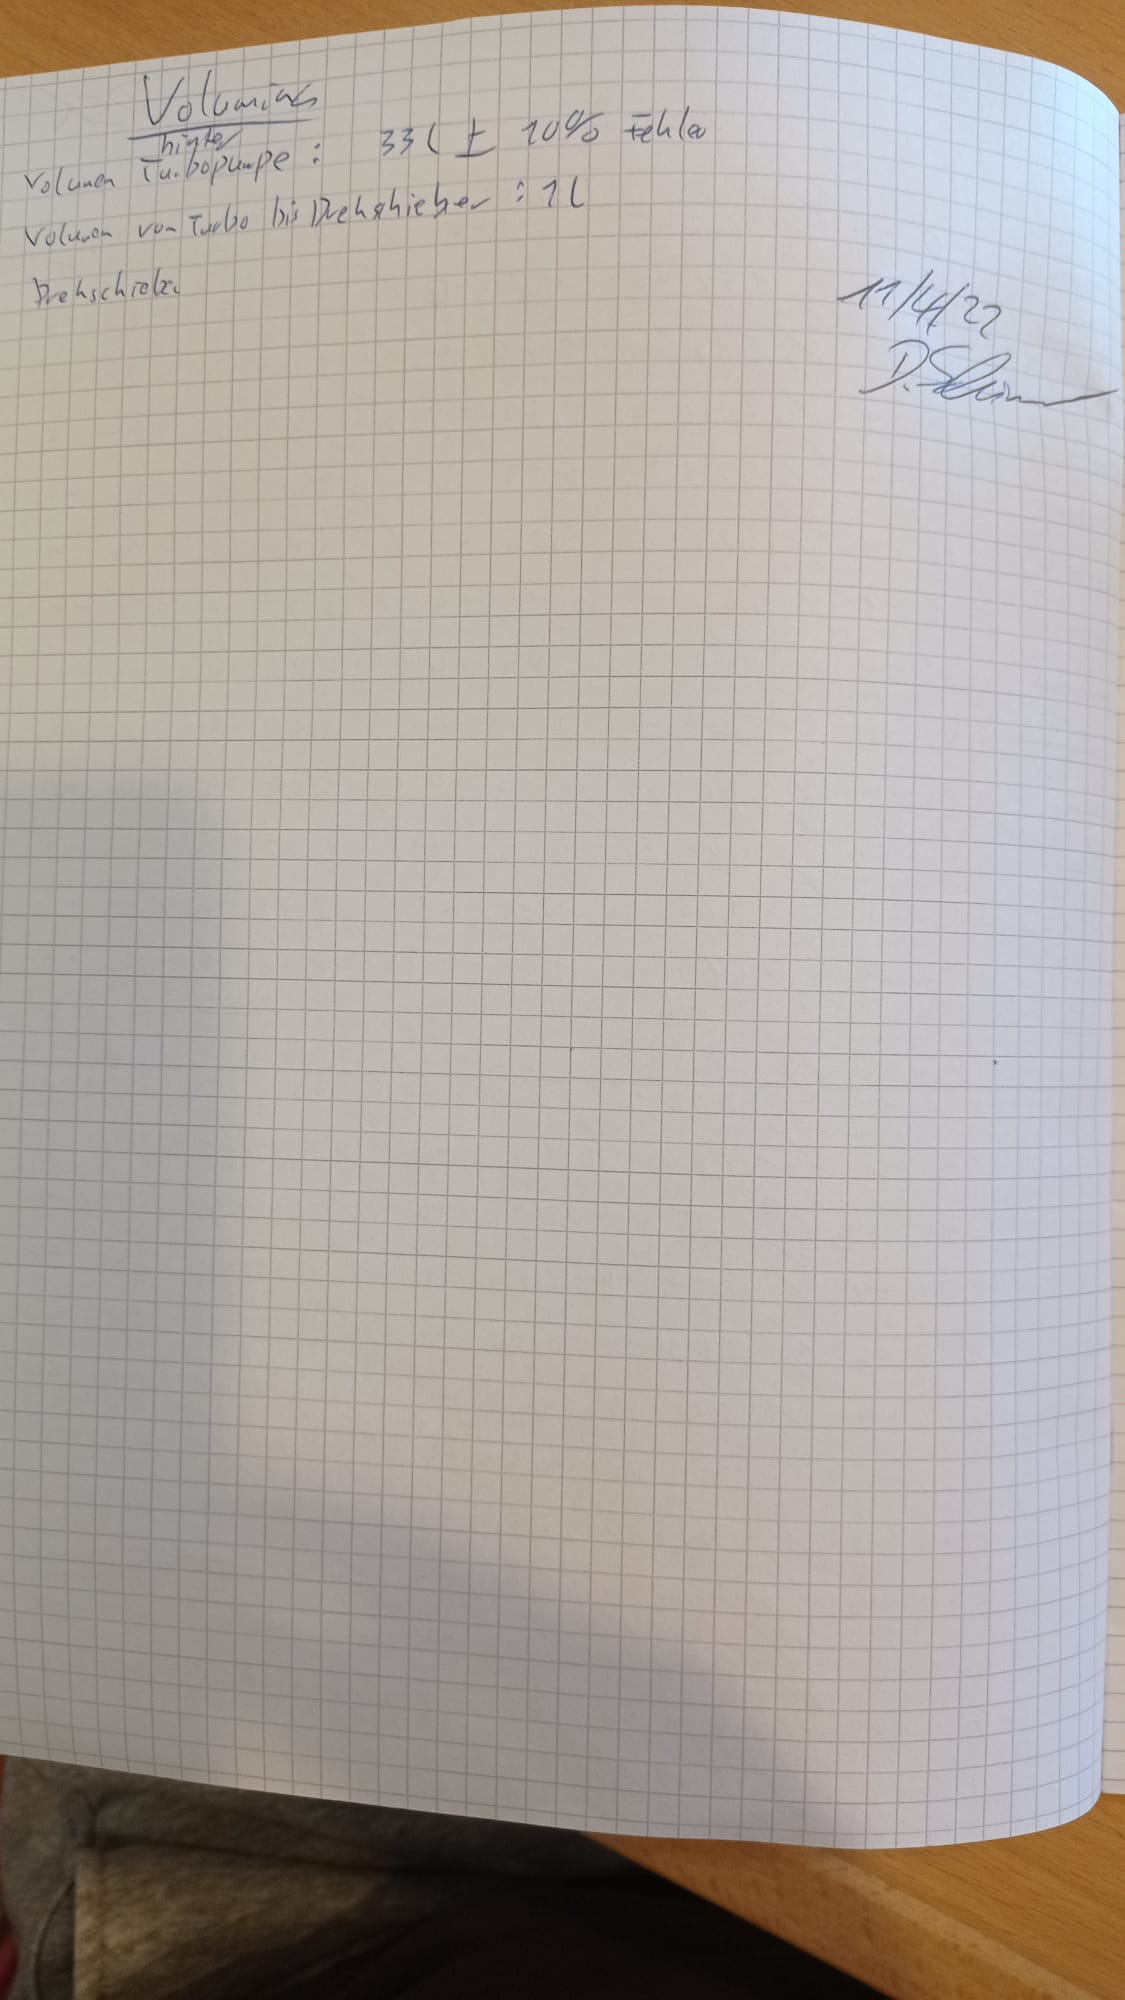
\includegraphics[width=0.7\textwidth]{latex/images/Messwerte_1.jpeg}
    \caption{Die Messwerte des Vakuumversuchs}
\end{figure}

\begin{figure}[h]
    \centering
    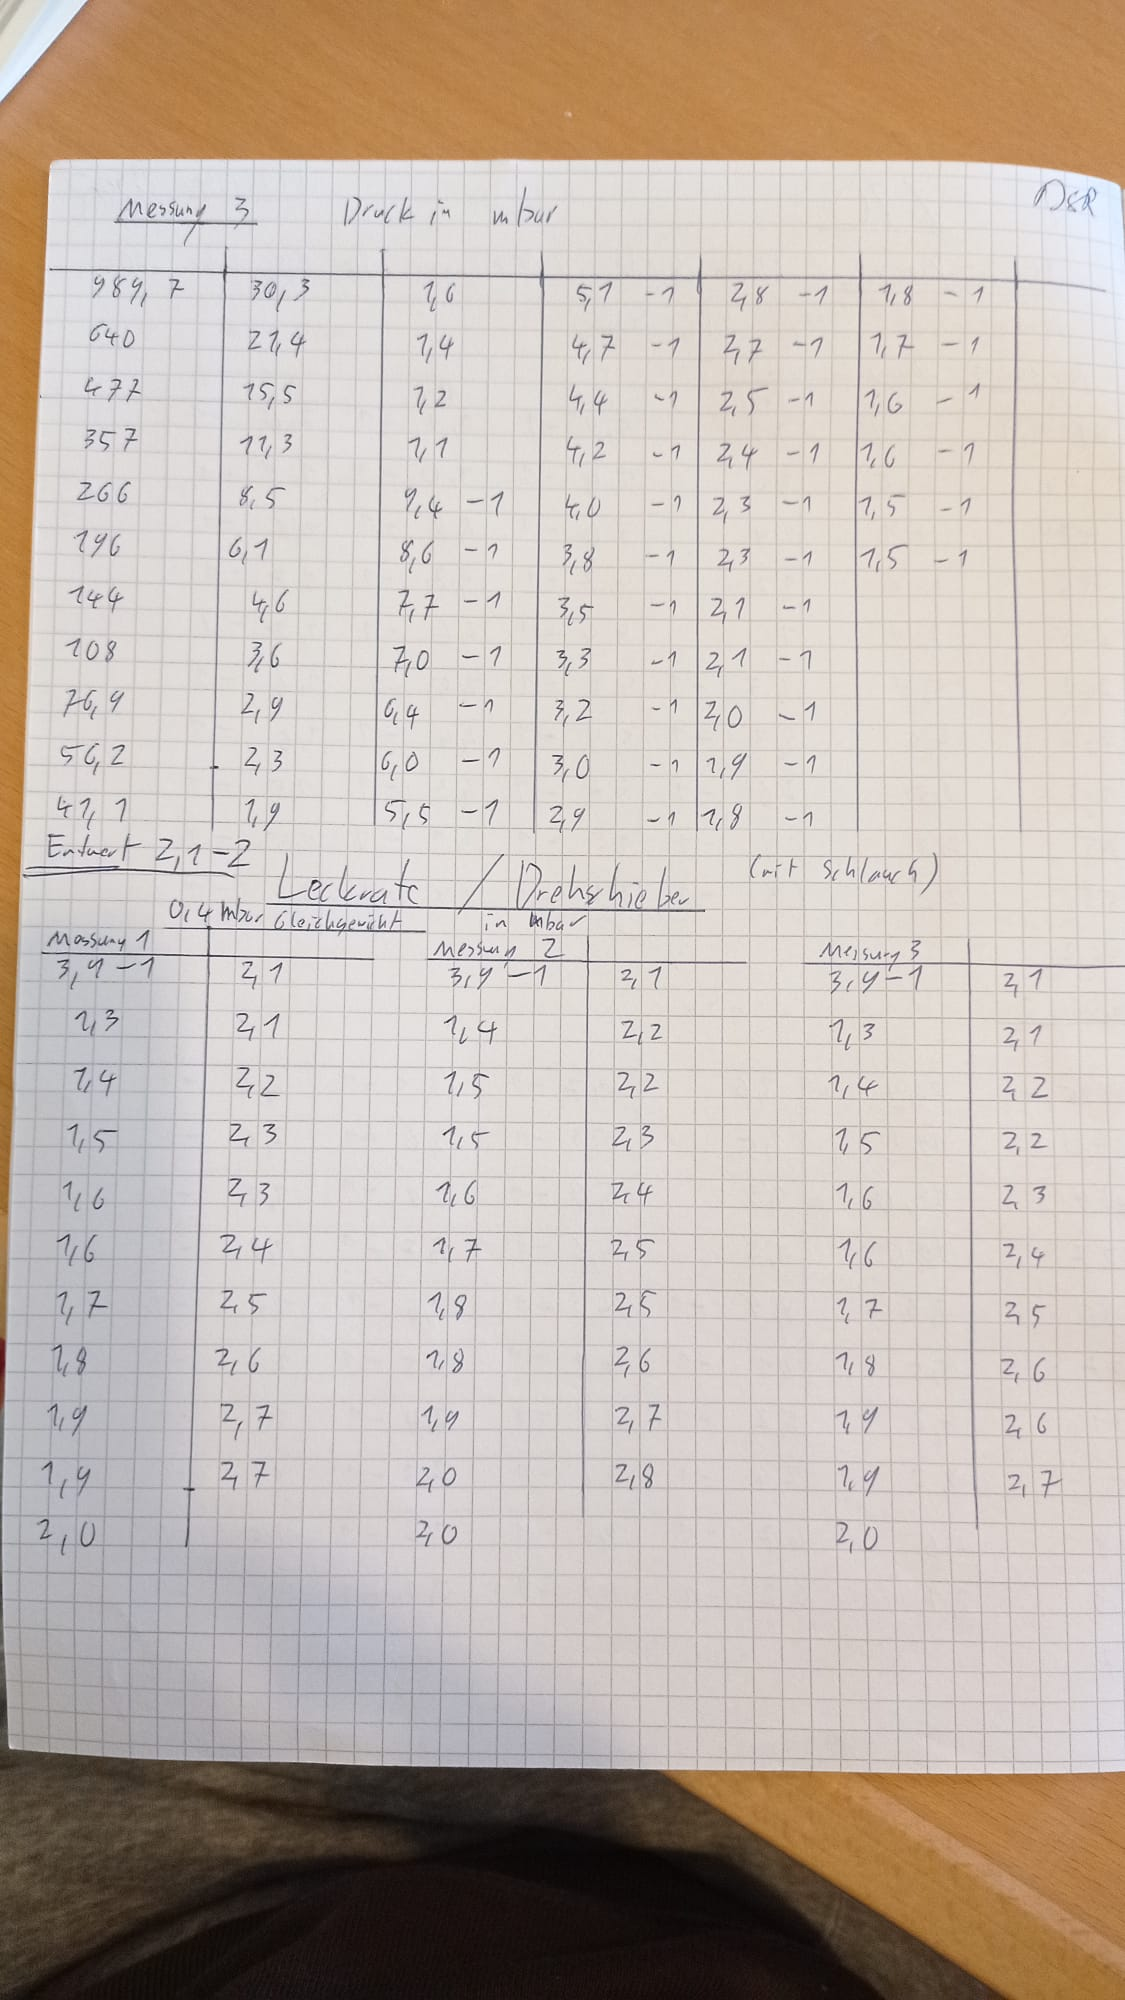
\includegraphics[width=0.7\textwidth]{latex/images/Messwerte_2.jpeg}
    \caption{Die Messwerte des Vakuumversuchs}
\end{figure}

\begin{figure}[h]
    \centering
    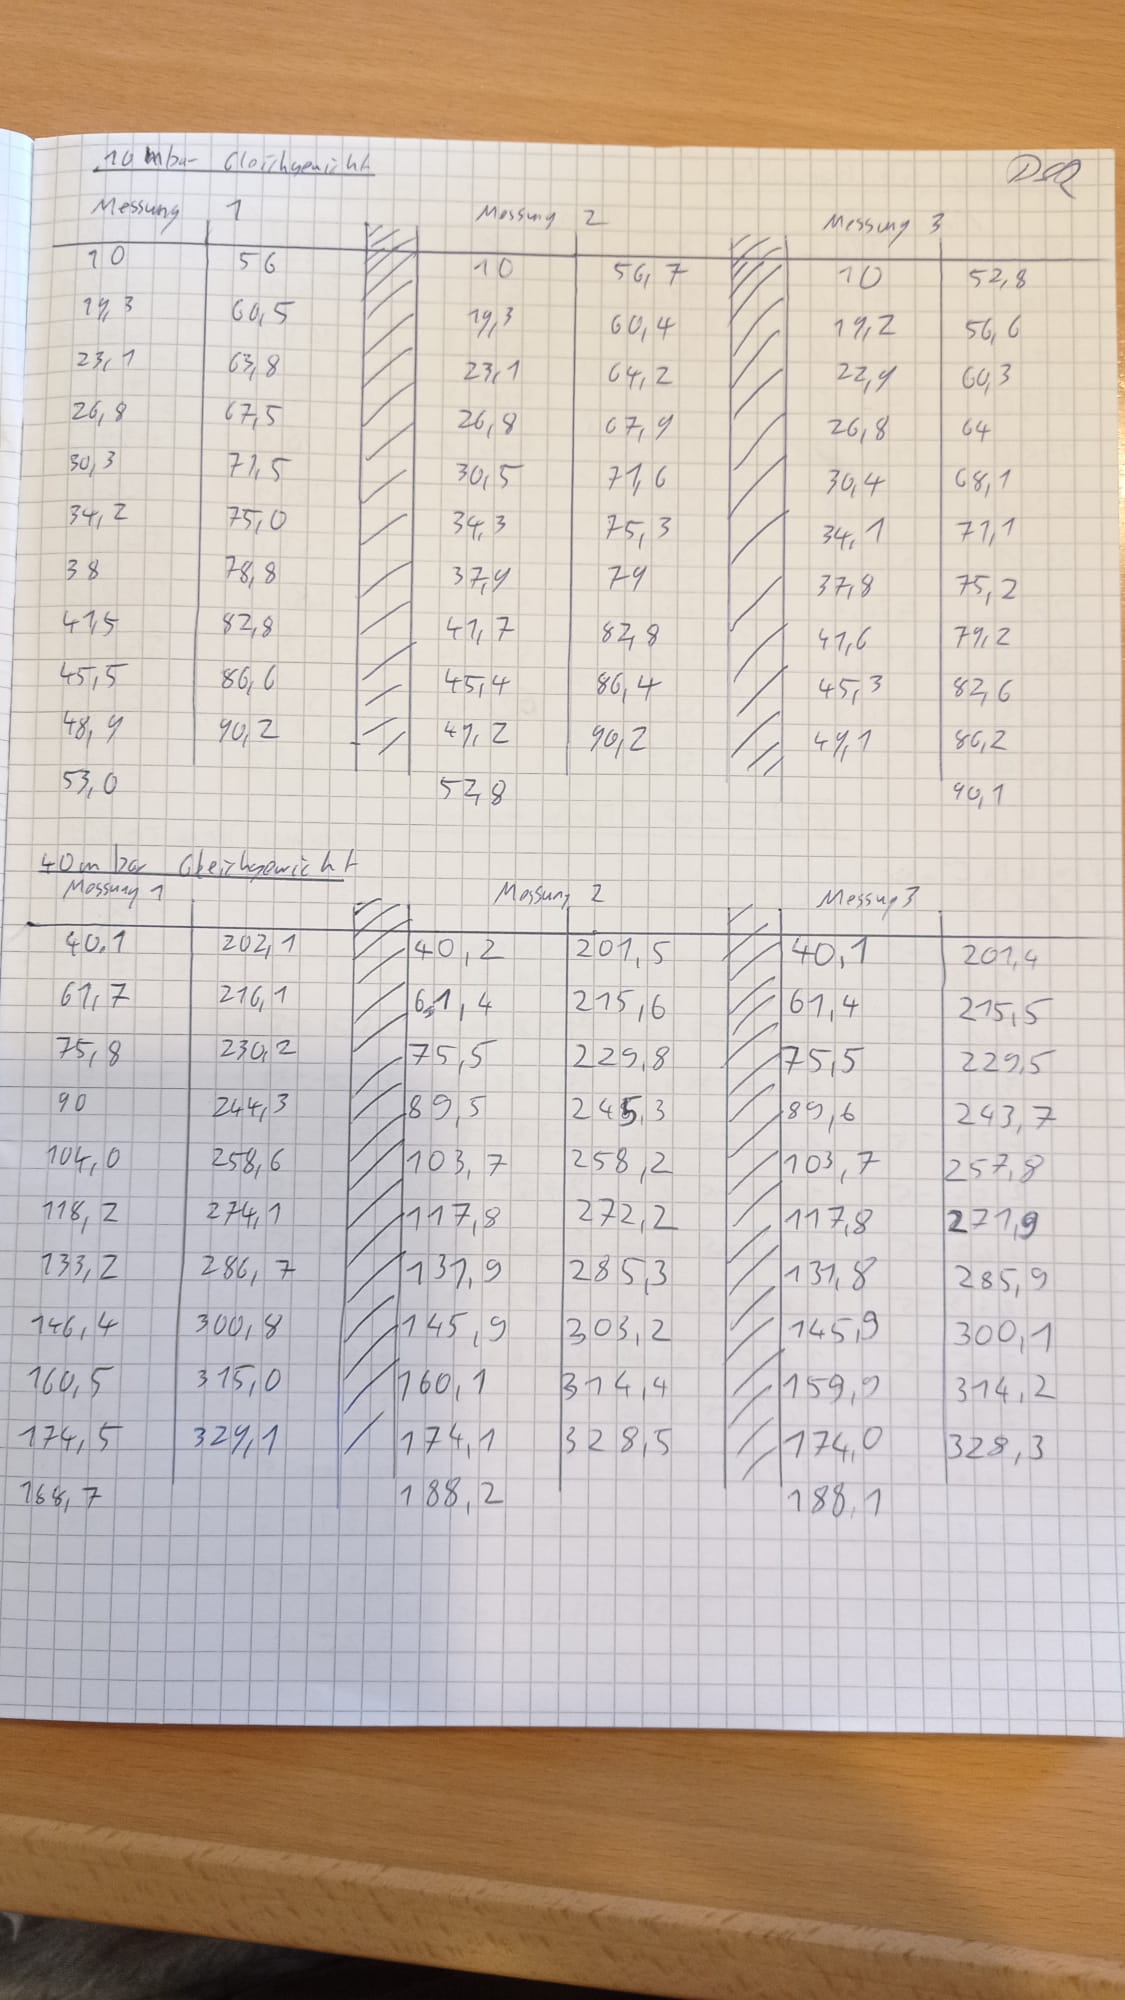
\includegraphics[width=0.7\textwidth]{latex/images/Messwerte_3.jpeg}
    \caption{Die Messwerte des Vakuumversuchs}
\end{figure}


\begin{figure}[h]
    \centering
    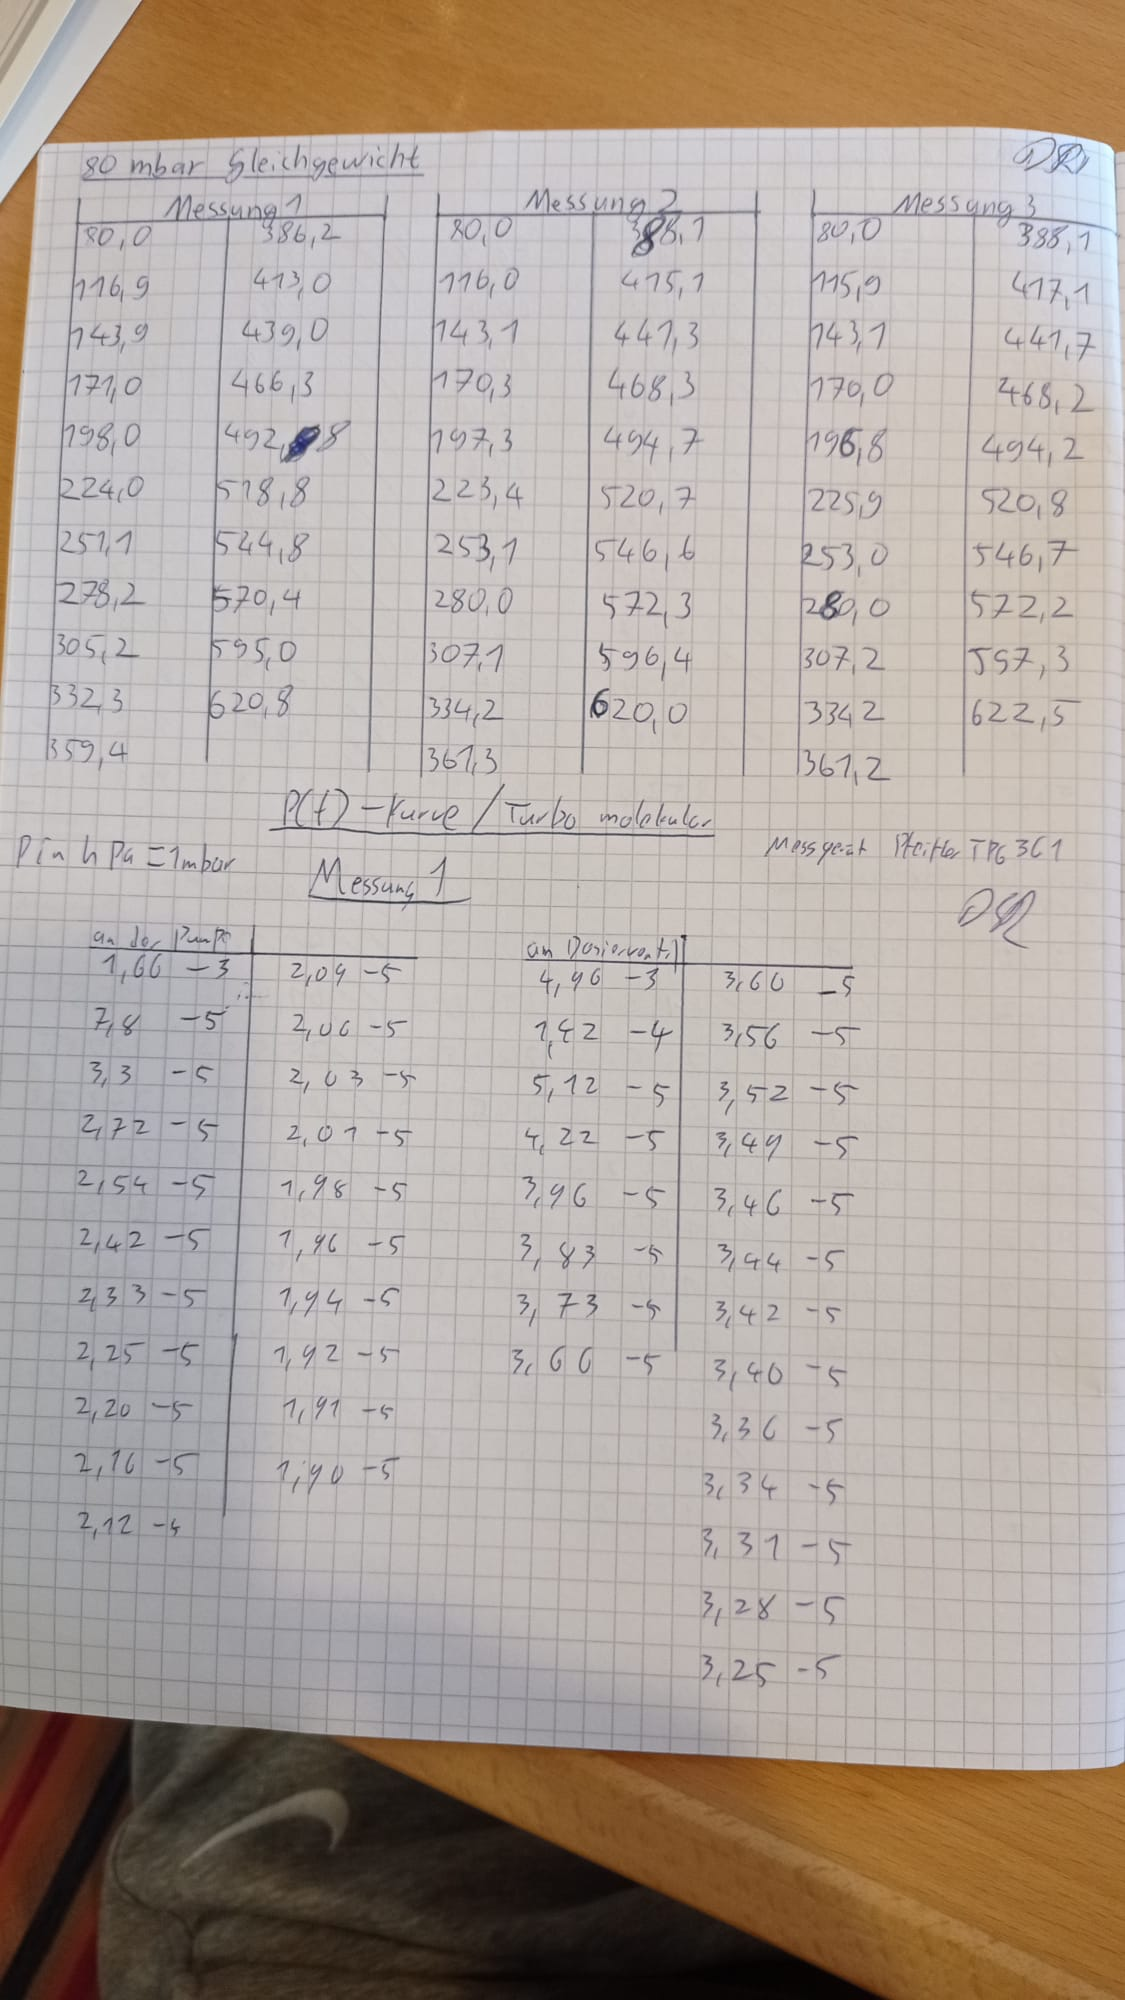
\includegraphics[width=0.7\textwidth]{latex/images/Messwerte_4.jpeg}
    \caption{Die Messwerte des Vakuumversuchs}
\end{figure}


\begin{figure}[h]
    \centering
    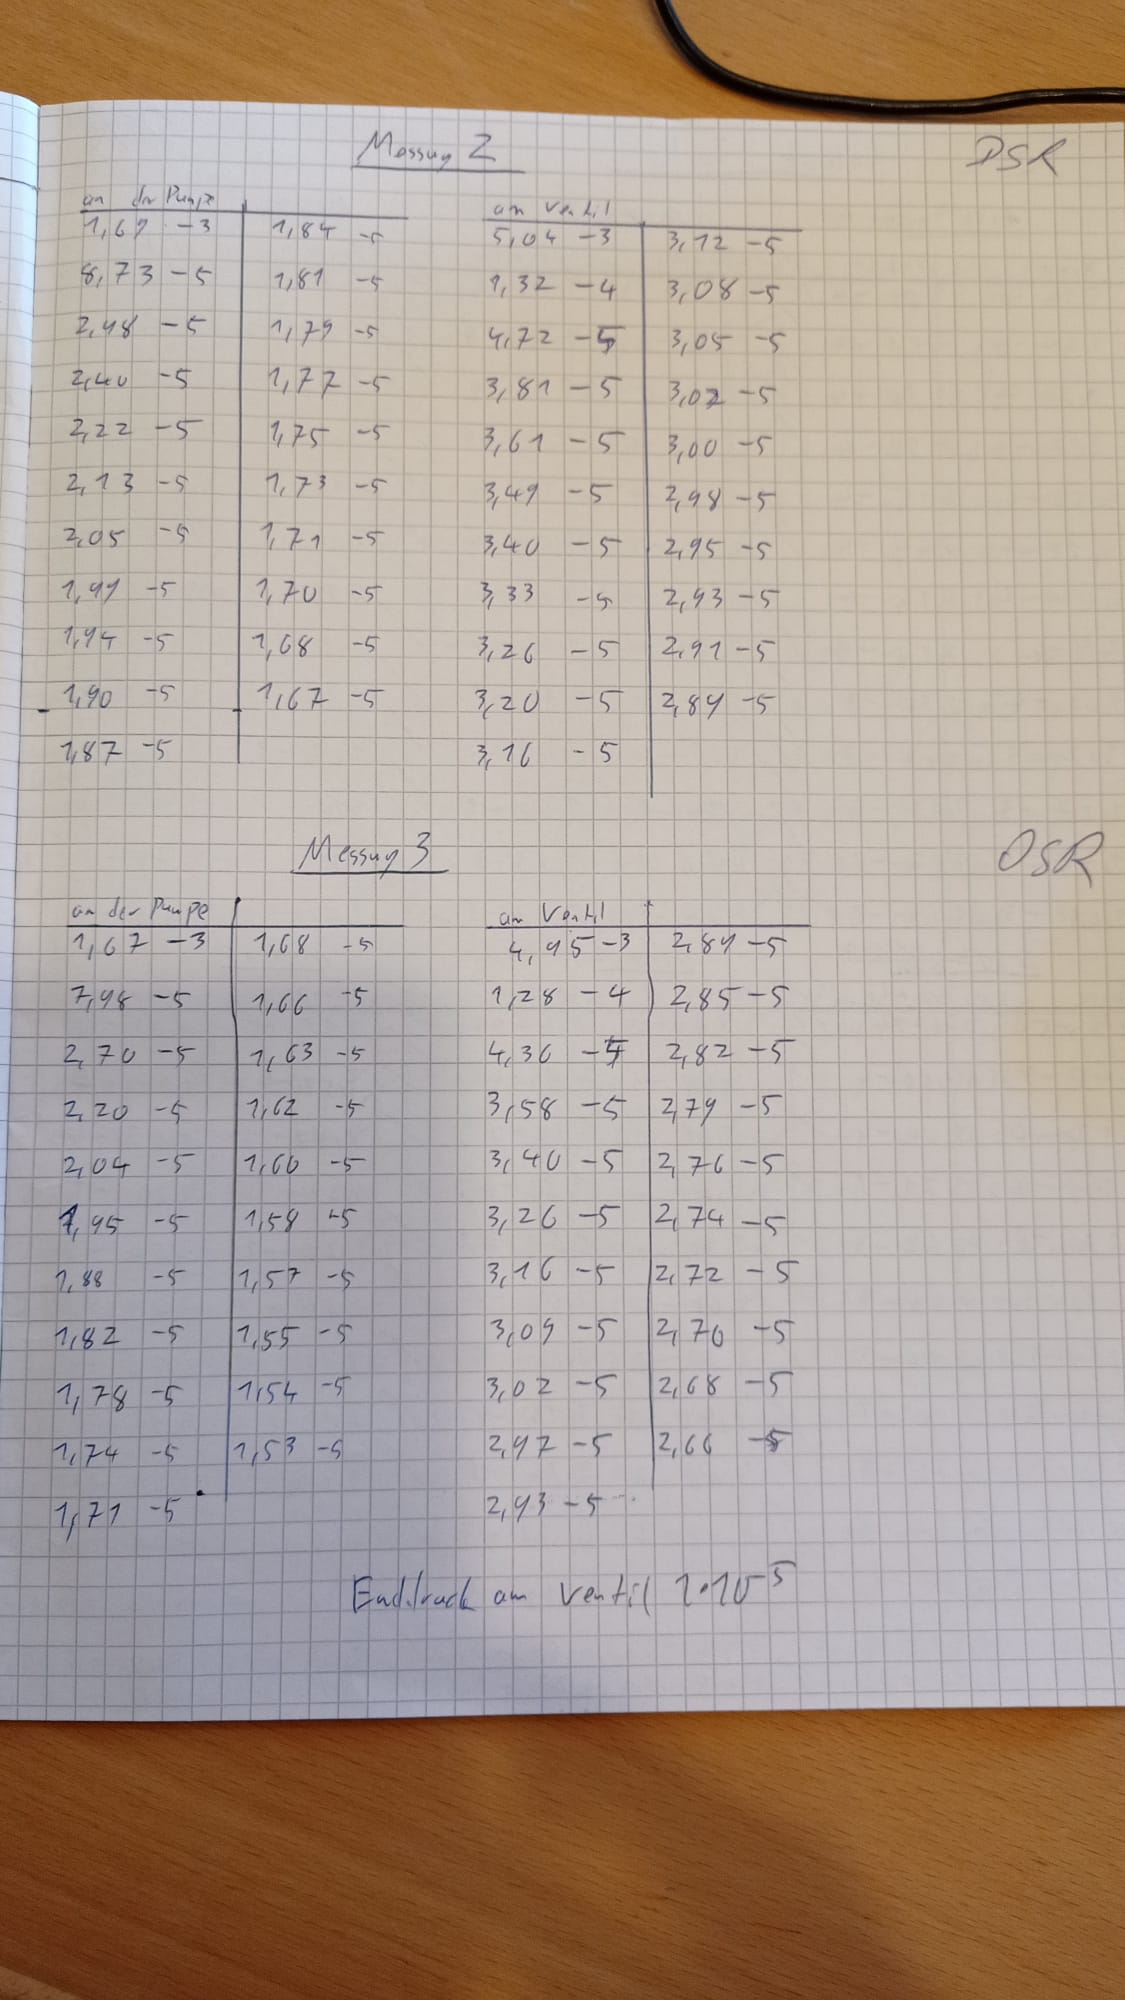
\includegraphics[width=0.7\textwidth]{latex/images/Messwerte_5.jpeg}
    \caption{Die Messwerte des Vakuumversuchs}
\end{figure}

\begin{figure}[h]
    \centering
    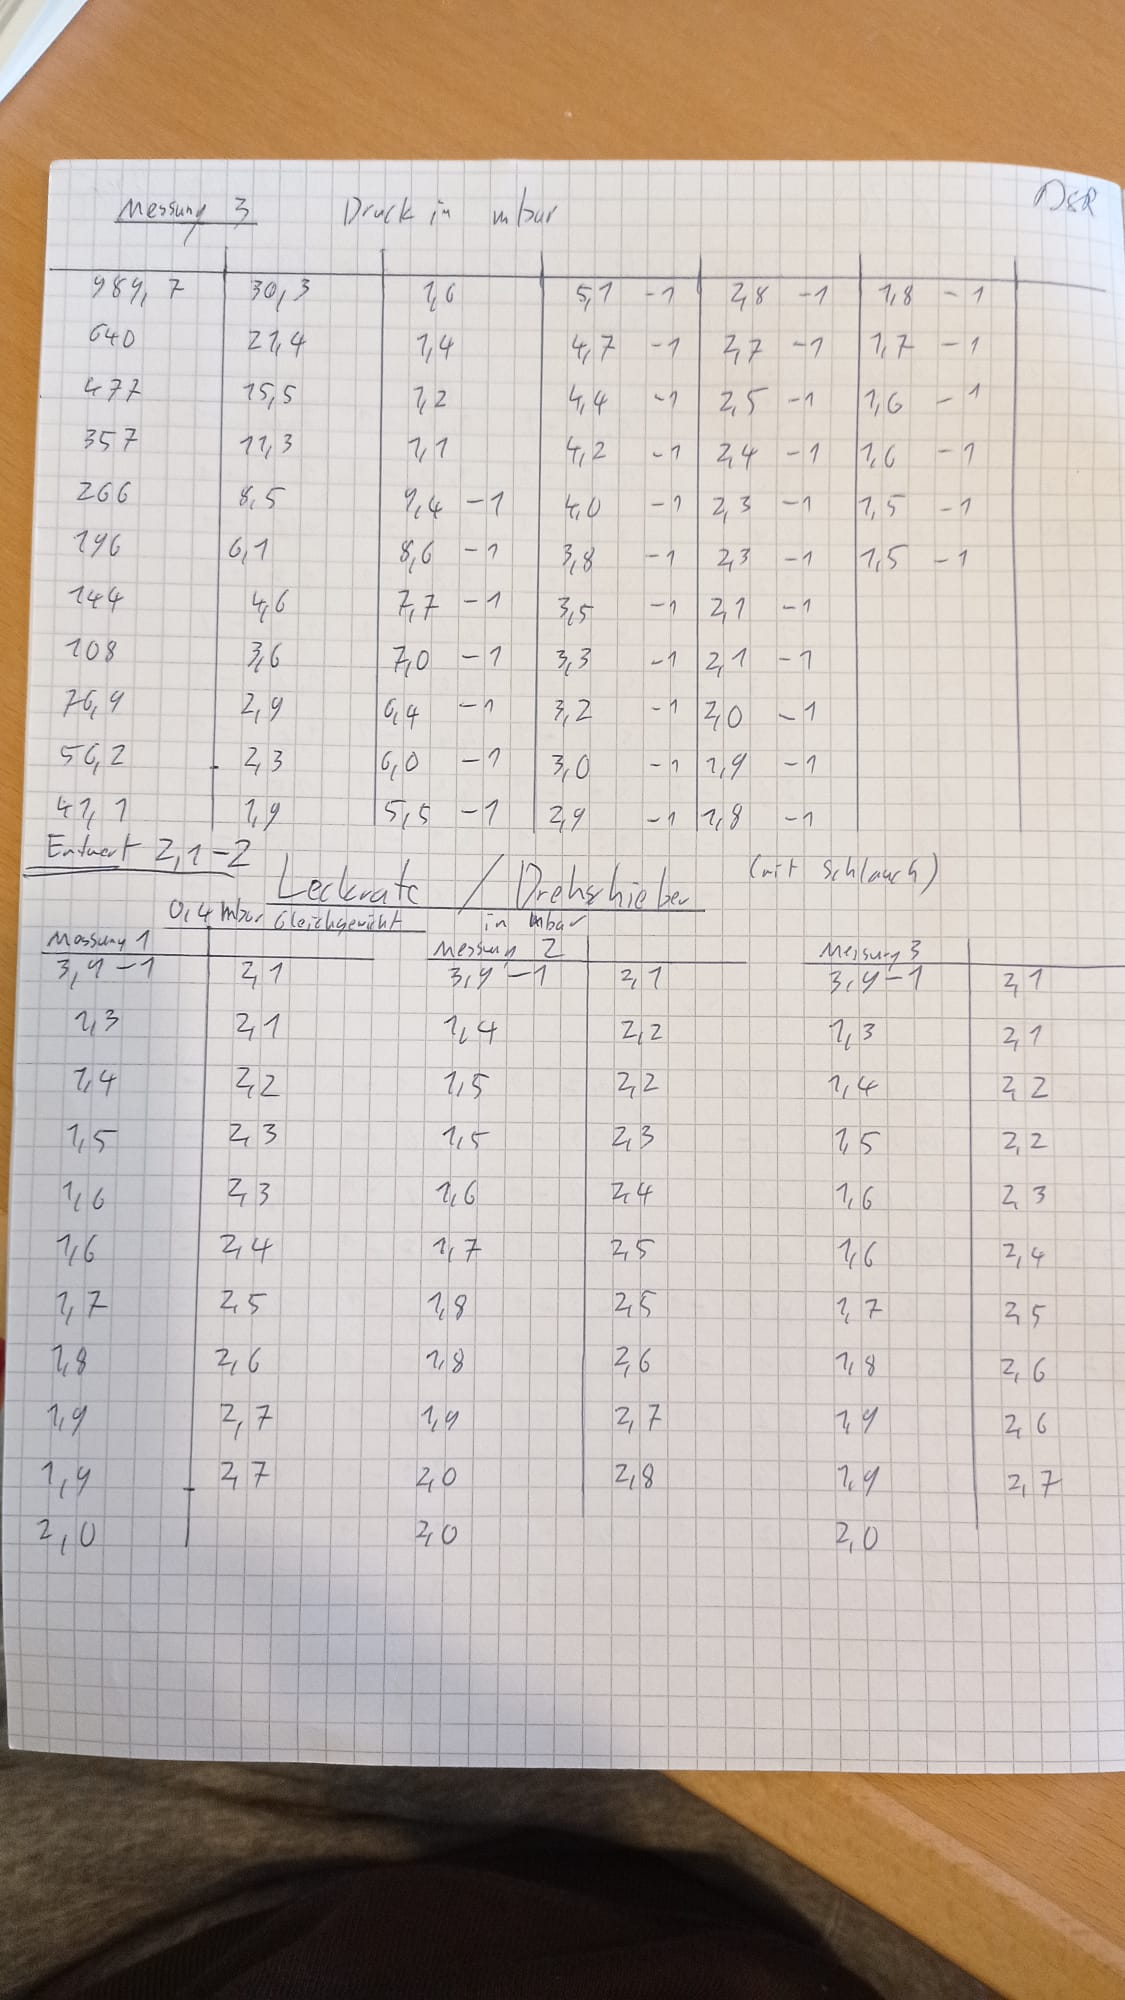
\includegraphics[width=0.7\textwidth]{latex/images/Messwerte_6.jpeg}
    \caption{Die Messwerte des Vakuumversuchs}
\end{figure}


\begin{figure}[h]
    \centering
    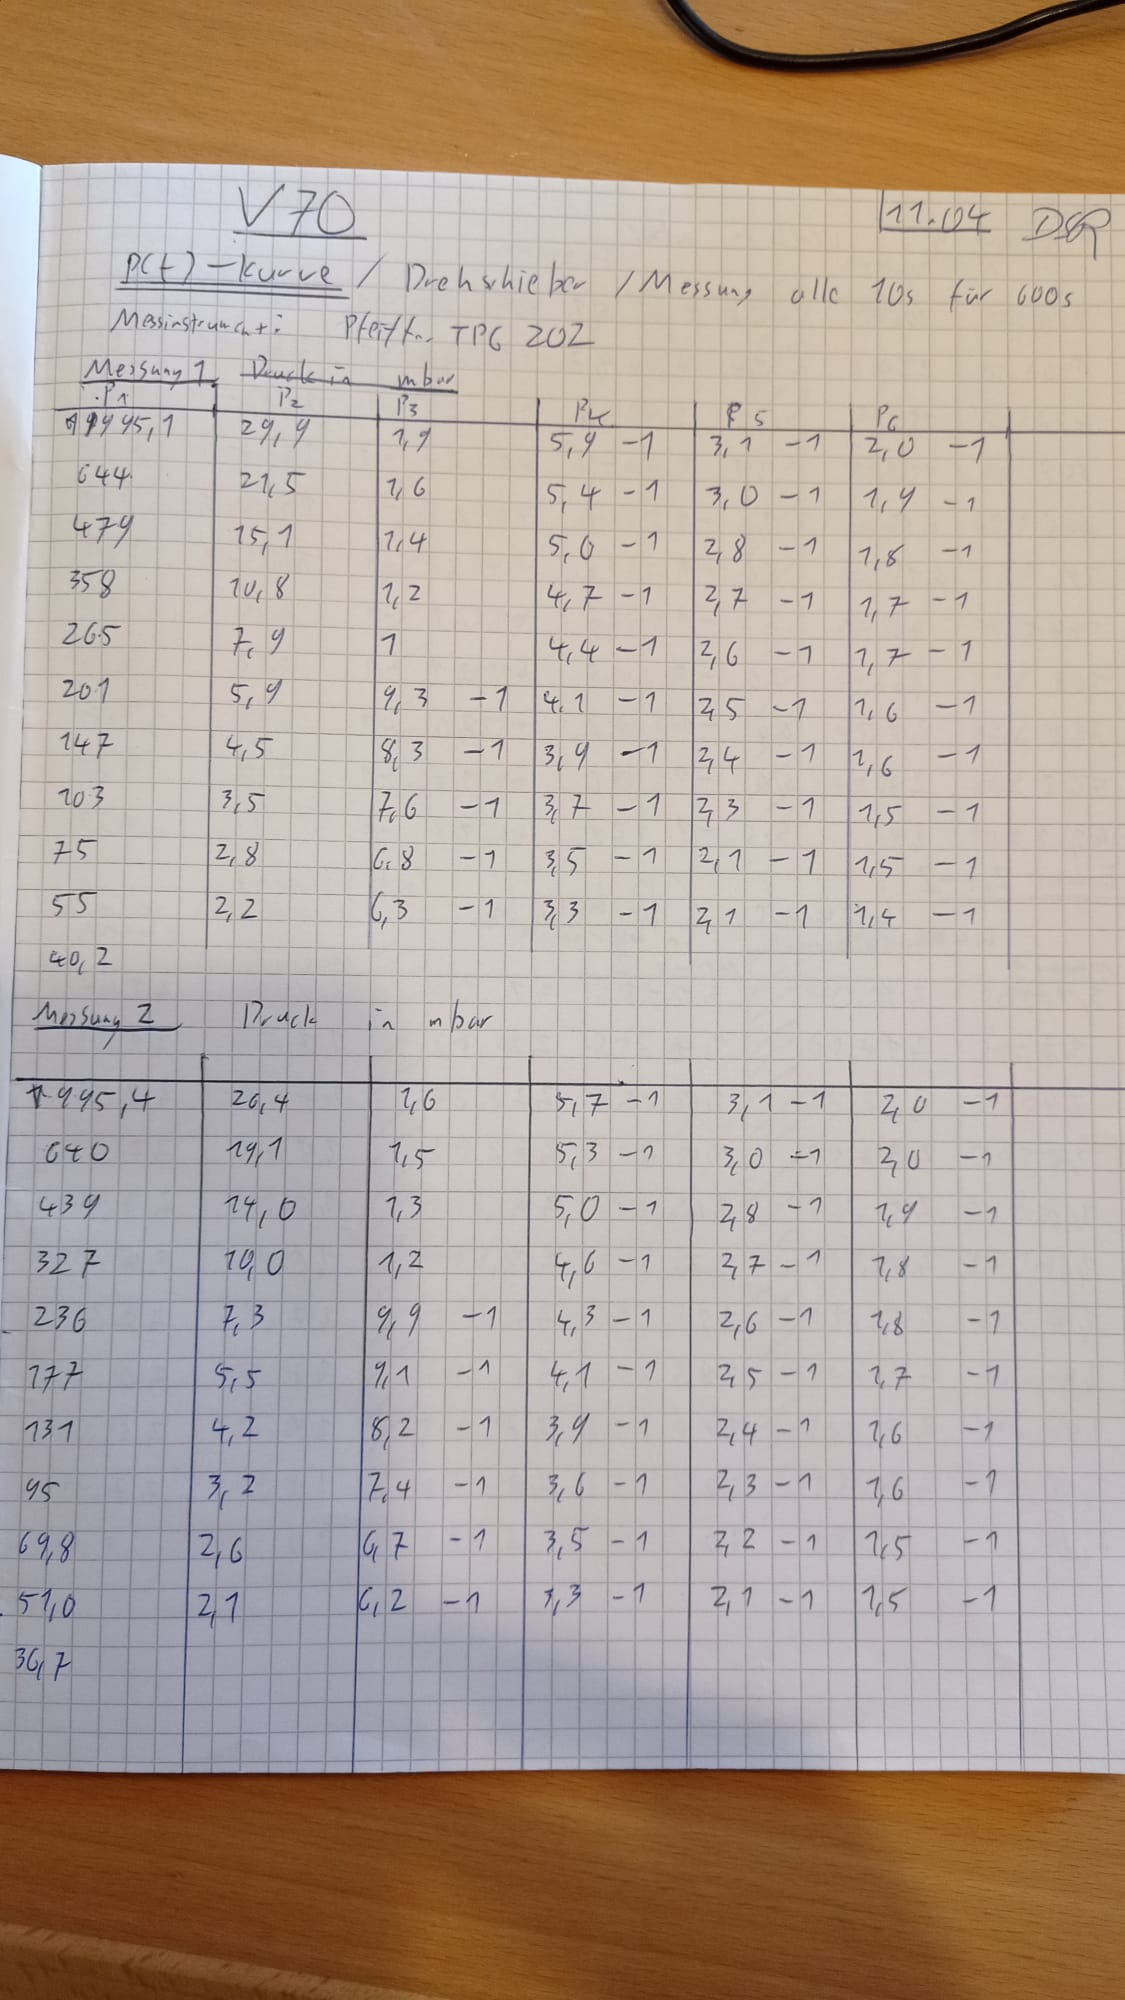
\includegraphics[width=0.7\textwidth]{latex/images/Messwerte_7.jpeg}
    \caption{Die Messwerte des Vakuumversuchs}
\end{figure}

\begin{figure}[h]
    \centering
    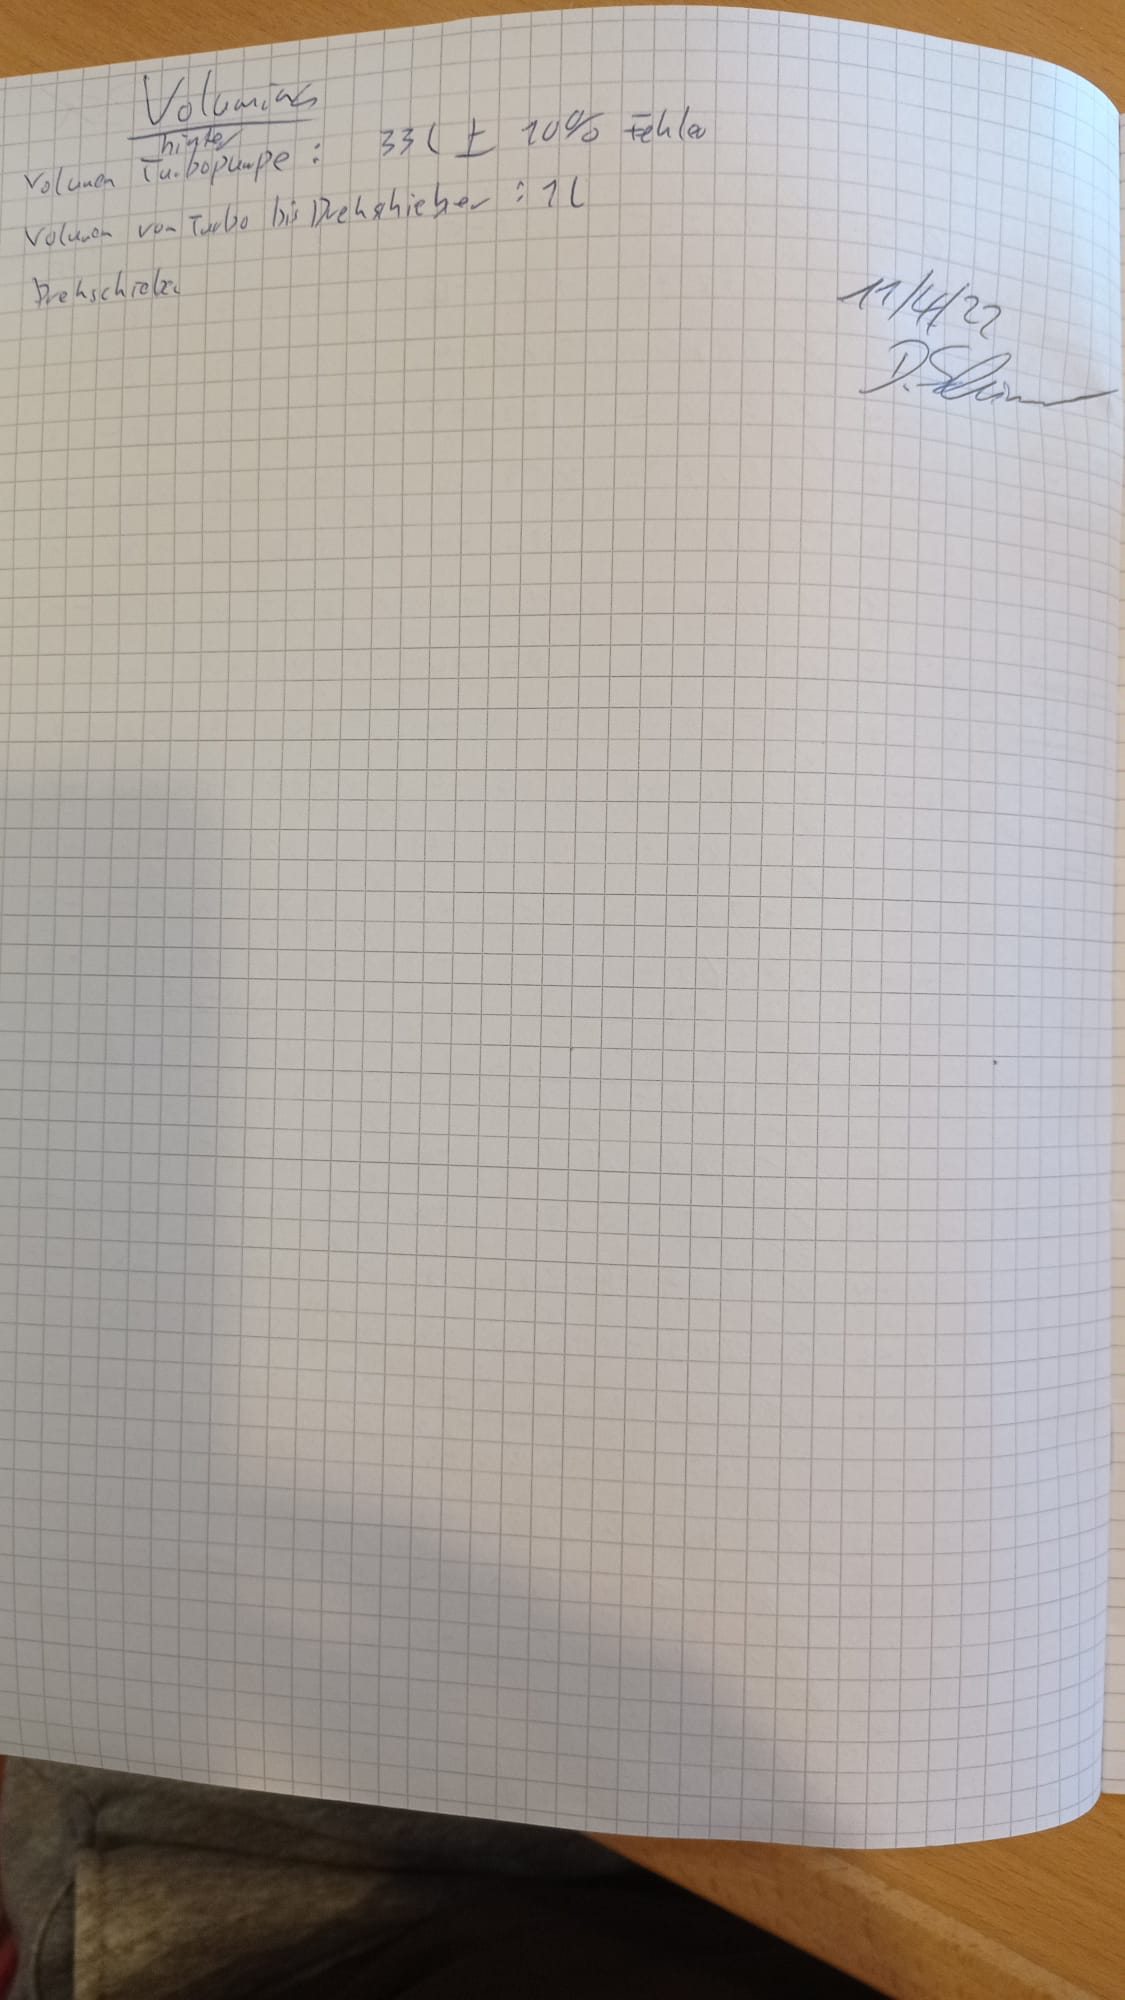
\includegraphics[width=0.7\textwidth]{latex/images/Messwerte_8.jpeg}
    \caption{Die Messwerte des Vakuumversuchs}
\end{figure}



